\documentclass[12pt, a4paper]{article}
\usepackage[utf8]{inputenc}
\usepackage{graphicx}
\graphicspath{{images/}}

\title{First document}
\author{Jovial Joe Jayarson \thanks{Ebin P M}}
\date{November 2020}

\begin{document}

\maketitle % This is needed for the title to be visible

First document. This is a simple example, with no extra parameters or packages included. We have now added a title, author and date to our first \LaTeX{} document!

% This line here is a comment, it will not be printed in the document.

Some of the \textbf{greatest} discoveries in \underline{science} were made by \textbf{\textit{accident}}. % What the \emph command actually does with its argument depends on the context - inside normal text the emphasized text is italicized, but this behavior is reversed if used inside an italicized text.

Some of the greatest \emph{discoveries} in science were made by accident.

\textit{Some of the greatest \emph{discoveries} in science were made by accident.}


The universe is immense and it seems to be homogeneous, in a large scale, everywhere we look at.

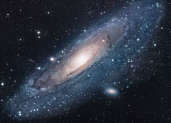
\includegraphics{universe} % no space between image names, good to omit extensions

There's a picture of a galaxy above.

\begin{figure}[h]
    \centering
    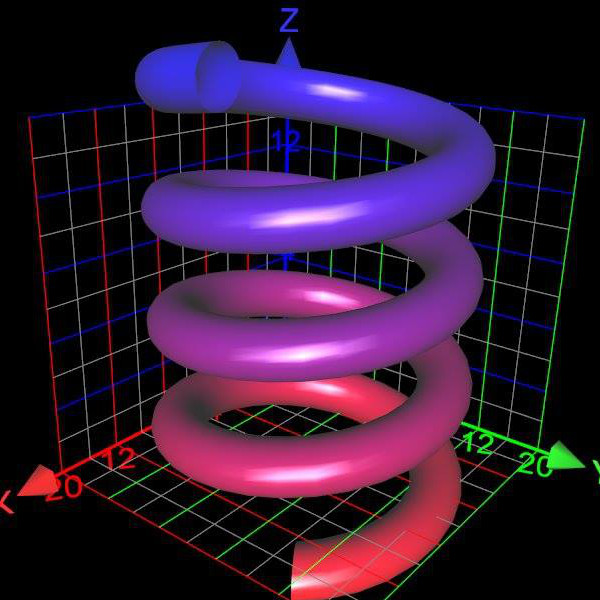
\includegraphics[width=0.25\textwidth]{graph}
    \caption{3D Circular Pipe}
    \label{fig:3D Torus}
\end{figure}

As you can see in the figure \ref{fig:3D Torus}, the function equivalent around 0. Also, in the page \pageref{fig:3D Torus} 
is the same example.

\end{document}
